\documentclass[a4paper]{article}

%% Language and font encodings
\usepackage[frenchb]{babel}
\usepackage[utf8x]{inputenc}
\usepackage[T1]{fontenc}
\usepackage{minted} %compiler avec la commande -shell-escape
\usepackage{graphicx}

%% Todo List
\usepackage{enumitem,amssymb}
\newlist{todolist}{itemize}{2}
\setlist[todolist]{label=$\square$}
\usepackage{pifont}
\newcommand{\cmark}{\ding{51}}%
\newcommand{\xmark}{\ding{55}}%
\newcommand{\done}{\rlap{$\square$}{\raisebox{2pt}{\large\hspace{1pt}\cmark}}%
\hspace{-2.5pt}}
\newcommand{\wontfix}{\rlap{$\square$}{\large\hspace{1pt}\xmark}}

%% Sets page size and margins
\usepackage[a4paper,top=3cm,bottom=2cm,left=3cm,right=3cm,marginparwidth=1.75cm]{geometry}
\setlength{\parskip}{.5em}

\newcommand{\HRule}{\rule{\linewidth}{0.5mm}}

%-------------------------------------------------------------------------------
% TITLE PAGE
%-------------------------------------------------------------------------------

\title
{
	\LARGE{Projet Technologique}
	\HRule \\ [0.5cm]
	\LARGE \textbf{\uppercase{Vision Stéréoscopique}}
	\HRule \\ [0.5cm]
}

\author{Geoffrey MEILHAN \\ Mohamed ALAMI CHENTOUFI \\ Kenji FONTAINE}

\begin{document}

\null  % Empty line
\nointerlineskip  % No skip for prev line
\vfill
\let\snewpage \newpage
\let\newpage \relax
\maketitle
\let \newpage \snewpage
\vfill
\break % page break

%-------------------------------------------------------------------------------
% Table of Contents
%-------------------------------------------------------------------------------

\tableofcontents
\newpage

%-------------------------------------------------------------------------------
% Introduction
%-------------------------------------------------------------------------------

\section{Description du projet}
La stéréoscopie est un ensemble de techniques visant à créer ou améliorer la
perception de relief à partir de deux images planes.

Le projet consiste à développer un module permettant d'évaluer une distance à
partir de deux images planes en entrée. Ce projet prendra la forme d'une implémentation
du module sur un système mobile à roues. L'objectif final étant de concevoir un robot
suiveur, capable de suivre une personne à une distance donnée.

%-------------------------------------------------------------------------------
% Domaine
%-------------------------------------------------------------------------------

\section{Domaine : Vision stéréoscopique}

Aujourd'hui devenu peu coûteux et peu encombrant, les systèmes de vision
stéréoscopiques sont de plus en plus répandus. \\
On trouve de nombreux domaines d'application dont les suivants :
\begin{itemize}
	\item Système de freinage automatique chez les voitures (Toyota par exemple).
	\item Détection d'obstacle chez les voitures autonomes.
	\item Reconnaissance d'objets chez les robots.
	\item La réalité virtuelle
\end{itemize}

%-------------------------------------------------------------------------------
% Cahier des charges
%-------------------------------------------------------------------------------

\section{Cahier des charges}

\subsection{Besoins fonctionnels}

Cette section décrit les besoins fonctionnels qui doivent être remplis par le
module crée.

\subsection*{OpenCV et QT}

Cette première partie décrit les besoins fonctionnels relatifs à la partie OpenCV
et QT du projet.

\subsubsection*{Split}

Le module doit pouvoir séparer verticalement une image en deux images de même taille.

\subsubsection*{Détection de bords}

Le module doit pouvoir détecter et mettre en valeur les bords d'une image.

\subsubsection*{Carte de disparité}

Le module doit pouvoir calculer une carte de disparité à partir de deux images
sources.

\subsubsection*{Carte de profondeur}

Le module doit pouvoir, à partir d'une carte de disparité, calculer une carte de
profondeur.

\subsubsection*{Conversion QImage/cv::Mat}

Le module doit pouvoir convertir une image d'un format à l'autre.

\subsection*{Unity}

\subsubsection*{Simulation}

L'environnement Unity doit permettre d'obtenir des images stéréoscopiques.

\subsection*{Robot}

\subsubsection*{Carte de profondeur}

Le robot doit pouvoir calculer une carte de profondeur à partir de deux images en
entrée en utilisant le module crée.

\subsubsection*{Estimer une distance}

Le robot doit pouvoir obtenir une distance à partir d'une carte de profondeur.

\subsubsection*{Déplacement}

Le robot doit pouvoir avancer ou reculer en fonction d'une distance estimée.

%-------------------------------------------------------------------------------
% Besoins non fonctionnels
%-------------------------------------------------------------------------------

\subsection{Besoins non fonctionnels}

\subsection*{OpenCV et QT}

\subsubsection*{Robuste}

Les distances estimées doivent être ordonnées de la même façon que les distances
réelles, sous des conditions variables de luminosité, ombres ou mouvements.

\subsubsection*{Rapide}

L'estimation de la distance doit être suffisament rapide afin de suivre une personne
marchant à vitesse normale (5km/h). Par manque de test, la rapidité n'est pas quantifiée.

\subsection*{Unity}

\subsubsection*{Automatisation}

L'acquisition d'image de synthèse doit être automatisable. Pour pouvoir prendre
plusieurs images d'un seul coup par exemple.

\subsection*{Robot}

\subsubsection*{Rapide}

L'estimation de la distance doit être suffisament rapide afin de suivre une personne
marchant à vitesse normale (5km/h). Par manque de test, la rapidité n'est pas quantifiée.

%-------------------------------------------------------------------------------
% Architecture du code QT CV
%-------------------------------------------------------------------------------

\section{Architecture du code : partie QT et OpenCV}

%%%%% CONVERT %%%%%
\subsubsection*{convert.cpp convert.h}

Ces fichiers permettent de convertir des images stockées sous le format d'openCV
(cv::Mat) en image sous format QT(QImage) et inversement. Il existe deux fonctions
principales : \textbf{mat2QImage} et \textbf{qImage2Mat}.

%%%%% EDIT %%%%%
\subsubsection*{edit.cpp edit.h}

Ces fichiers forment le "core" de notre module. Sont incluent la plupart des
algorithmes utilisés lors des calculs de carte de disparité ou de profondeur,
de détection de bords, de détections de points d'intérêt, etc...


\textbf{split :} Cette fonction permet de séparer verticalement une image en
entrée, en deux images de même taille. Elle prend en entrée une image de type
QImage. Cette QImage sera coupée en deux et chaque partie ainsi obtenue sera
respectivement stockée dans les cv::Mat dont les adresse sont données en paramètres.


\textbf{sobel :} Cette fonction permet de détecter les bords d'une image. Elle
prend en entrée une image de type cv::Mat. la fonction va effectuer sur l'image
source une détection de bords, puis stockera le résultat ainsi obtenu dans une
autre image cv::Mat dont l'adresse est donnée en tant que paramètre.


\textbf{surf et surfmatch :} Ces deux fonctions permettent d'effectuer une détection
de points d'intérêts. La fonction \textbf{surf} prend une seule image de type
cv::Mat en entrée. Elle va détecter les points d'intérêt sur l'image en entrée puis
les mettre en valeur. Le résultat obtenu sera stockée dans une autre image cv::Mat
dont l'adresse est donnée en tant que paramètre.


La fonction \textbf{surfMatch} fait la même chose mais avec 2 images en entrée,
toujours de type cv::Mat. Elle va, en plus de la détection de points d'intérêts,
effectuer une mise en correspondance des points d'intérêts entre eux. Le résultat
obtenu sera stocké dans une cv::Mat de destination dont l'adresse est en paramètre
de la fonction.


\textbf{dispMap :} Cette fonction permet de calculer une carte de disparité à
partir de deux images cv::Mat en entrée. Elle fait appel à l'algorithme
\textbf{StereoBM} de la bibliothèque \textbf{OpenCV}. La carte de disparité ainsi
obtenue est stockée dans une image cv::Mat dont l'adresse est donnée en paramètre.

%%%%% MAIN %%%%%
\newpage
\subsubsection*{main.cpp}

Il s'agit du code exécuté lors du lancement du programme. On distingue 2 parties.
Une première partie avec GUI correspond au code généré par défaut par QT.
Elle permet de lancer le programme avec l'interface graphique.

\begin{minted}{cpp}
int main(int argc, char *argv[])
{
	QApplication a(argc, argv);
	MainWindow w;
	w.show();

	return a.exec();
}
\end{minted}

Une deuxième partie permet d'executer des parties différentes du code en fonction de l'argument rentré lors de l'appel du programme. Si l'appel au programme se fait par la commande:
\begin{minted}{bash}
$ ./projet 0
\end{minted}
Alors le programme va traiter toutes les images dans les sous-dossiers écrits en dur dans le code, dans ce cas précis il récupère les images dans le dossier source/cam et écrit dans le dossier result/cam avec l'appel suivant:
\begin{minted}{cpp}
for (int j = 0 ; j < 3 ; j++) {
  for (int i = 0 ; i < 5 ; i++) {
    std::ostringstream ossI, ossO;
    ossI << "source/cam" << j << "-dist" << i << ".png"; //path fichier entrant
    ossO << "result/cam" << j << "-dist" << i << ".png"; //path fichier sortant
\end{minted}
Le nombre d'images traitée est i*j et est rentré en dur dans le code. Cette partie a été écrite pour faciliter le traitement d'un grand nombre d'images, afin de tester les cartes de profondeur sur diverses situations.

Une troisième partie très similaire à celle décrite plus haut, à la différence pret que les images en entrée sont au nombre de deux et ont déjà était split. L'implémentation est la même avec la quantitée d'images écrite en dur dans le code, tout comme les dossiers contenant les images. L'appel se fait par:
\begin{minted}{bash}
$ ./projet 1
\end{minted}

Enfin un dernier appel au programme peut être fait permettant de tester plusieurs valeurs de SADWindowSize et de ndisparities pour une image rentrée dans le code. Celà nous a permis de faire des tests sur les valeurs optimales de StereoBM sur une certaine image, avant notre implémentation des trackbars. L'appel se fait par:
\begin{minted}{bash}
$ ./projet 2
\end{minted}

%%%%% SGBM %%%%%
\subsubsection*{sgbm.cpp sgbm.h}

Ces fichiers contiennent les deux fonctions permettant de créer l'interface dynamique
de gestion des paramètres du calcul de carte de disparité. \\
\textbf{dispSGBM :} Cette fonction charge des images sources en mémoire, initialise
les paramètres de calcul de l'algorithme SGBM ainsi que les trackbars permettant de
modifier dynamiquement les paramètres. \\
\textbf{update :} Cette fonction permet de mettre à jour les paramètres lorsque
l'utilisateur agit sur une des trackbars. Elle rafraichit également l'affichage des
cartes de disparité.

%-------------------------------------------------------------------------------
% Architecture du code Unity
%-------------------------------------------------------------------------------

\newpage
\section{Architecture du code : partie Unity}

\subsection*{move.cs}

Ce script permet à l'objet auquel il est attaché de se déplacer dans une scène
Unity en utilisant les flèches directionnelles. Par exemple, le code suivant est
exécuté lorsque l'utilisateur appuie sur la flèche avant.
\begin{minted}{csharp}
	if (Input.GetKeyDown (KeyCode.UpArrow)) {
		Vector3 position = this.transform.position;
		position.y++;
		this.transform.position = position;
	}
\end{minted}

\subsection*{capture.cs}

Pour que ce script fonctionne il faut qu'il y ait 3 objets avec les tags suivant :
camera\_left, camera\_right, bob. Ce script est à attacher à n'importe quel objet
d'une scène. Ce script va déplacer les objets et rendre en tant qu'image la vue des
caméras. \\
Dans notre simulation, camera\_left et camera\_right représentent nos caméras stéréo
et bob représente un humain à une certaine distance de ces caméras. Le script
permet de prendre des captures d'écran en faisant varier la distance entre les caméras
ainsi que la distance caméras-humain. \\
Voici la boucle principale du script :
\begin{minted}{csharp}
	for (int j = 0; j < 3; j++) {
		for (int i = 0; i < 5; i++) {
			// Render a picture and save it
			move ("bob", 'z', 1); // Move object with tag "bob"
		}
		// reset bob to initial position and move each camera
		reset ("bob", initial);
		move ("camera_left" , 'x', -0.02f);
		move ("camera_right", 'x',  0.02f);
	}
\end{minted}


%-------------------------------------------------------------------------------
% Tests
%-------------------------------------------------------------------------------

\newpage
\section{Tests}

\subsection*{Ouverture d'une image}

Pour ouvrir une image, il faut aller dans le menu \textbf{File} puis appuyer sur
"Open File". \\[0.4cm]
\centerline{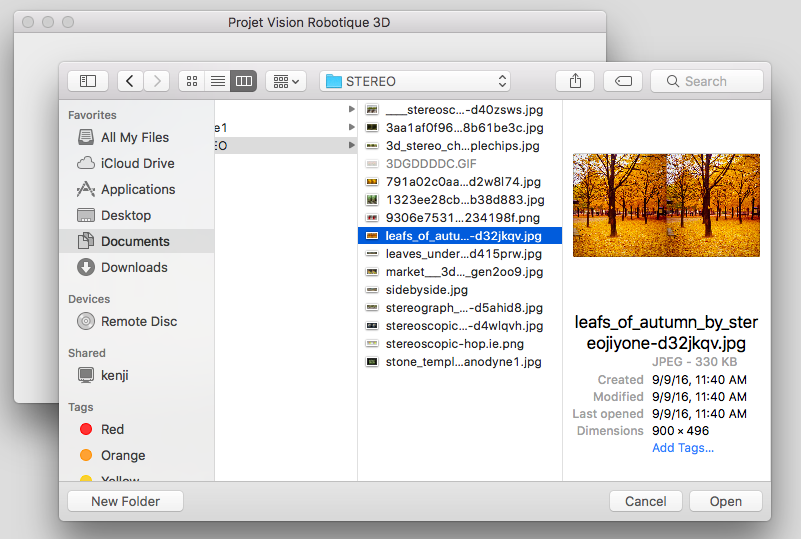
\includegraphics[width=\textwidth,height=\textheight,keepaspectratio]{img/1.png}}

Et le résultat : \\[0.4cm]
\centerline{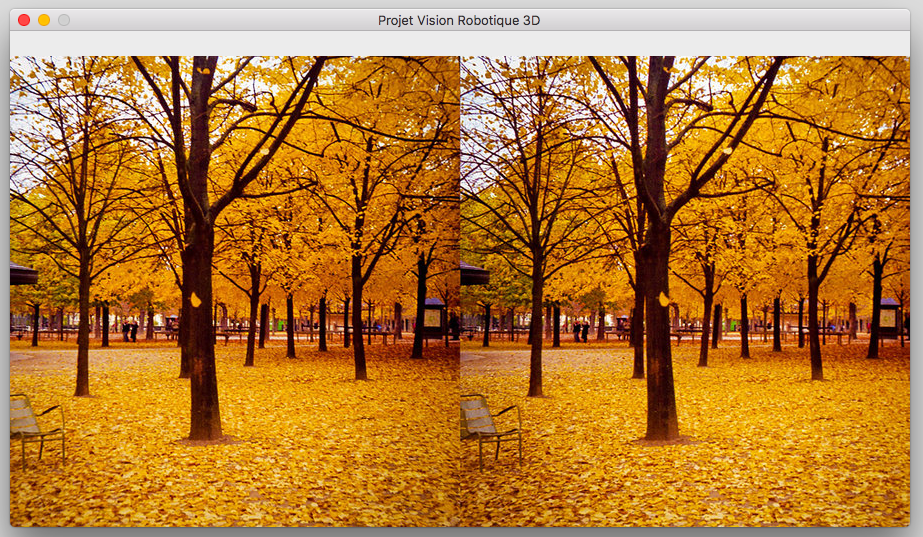
\includegraphics[width=\textwidth,height=\textheight,keepaspectratio]{img/2.png}}

\subsection*{Conversion de format}

Pour convertir une image, il faut en avoir une d'ouverte. Puis aller dans le menu
\textbf{Edit} et cliquer sur "Convert test". Cette fonction va convertir l'image de
base, chargée comme QImage, en cv::Mat puis la reconvertir en QImage avant de
l'afficher. Cela permet de tester la conversion dans les deux sens.

\subsection*{Split}

Pour séparer une image en deux, il faut tout d'abord en avoir ouvert une. Puis
aller dans le menu \textbf{Edit} et cliquer sur "Split test". \\
Voici le résultat obtenu : \\[0.4cm]
\centerline{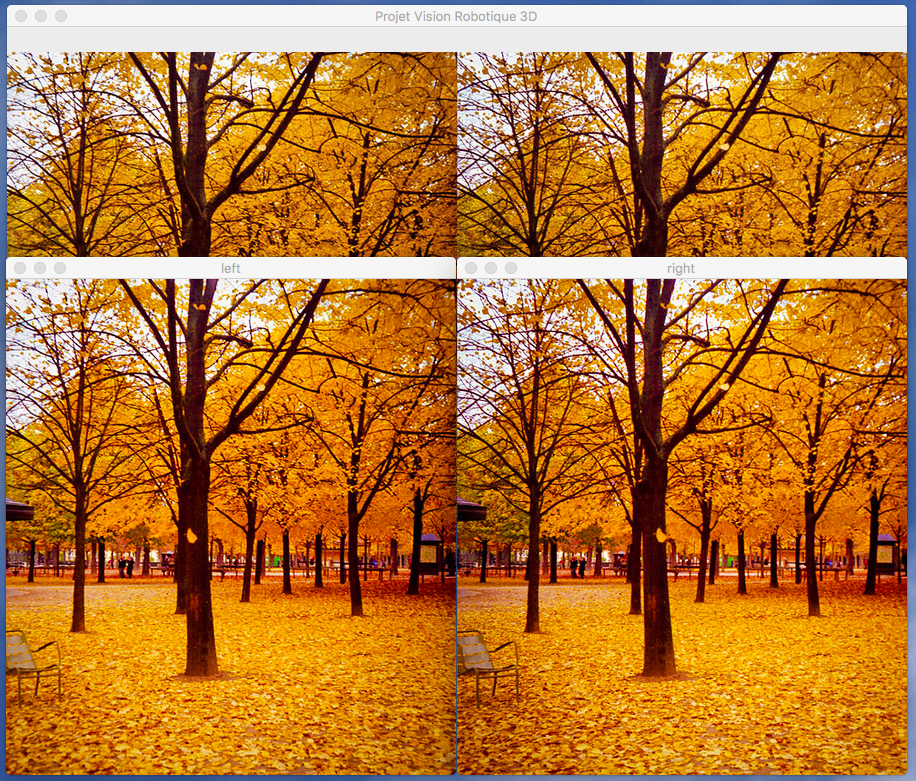
\includegraphics[width=\textwidth,height=\textheight,keepaspectratio]{img/3.png}}

\newpage
\subsection*{Détection de bords}

Pour effectuer une mise en valeur des bords d'une image, aller dans le menu
\textbf{Edit} et cliquer sur \textbf{Sobel test}. \\
Voici le résultat obtenu : \\[0.4cm]
\centerline{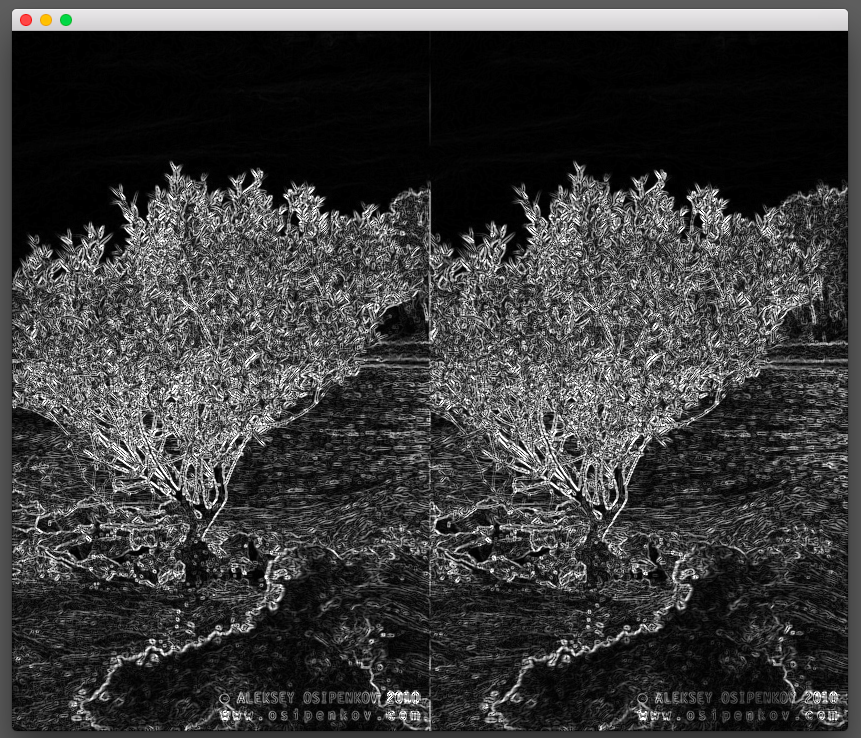
\includegraphics[width=\textwidth,height=\textheight,keepaspectratio]{img/4.png}}

\newpage
\subsection*{Carte de disparité}

Pour afficher une carte de disparité, il faut ouvrir une image. Puis, aller dans
le menu \textbf{Edit} et appuyer sur "Disp map test". La séparation verticale est
automatique, il n'est pas nécessaire de "split" l'image avant. \\
Et le résultat : \\[0.4cm]
\centerline{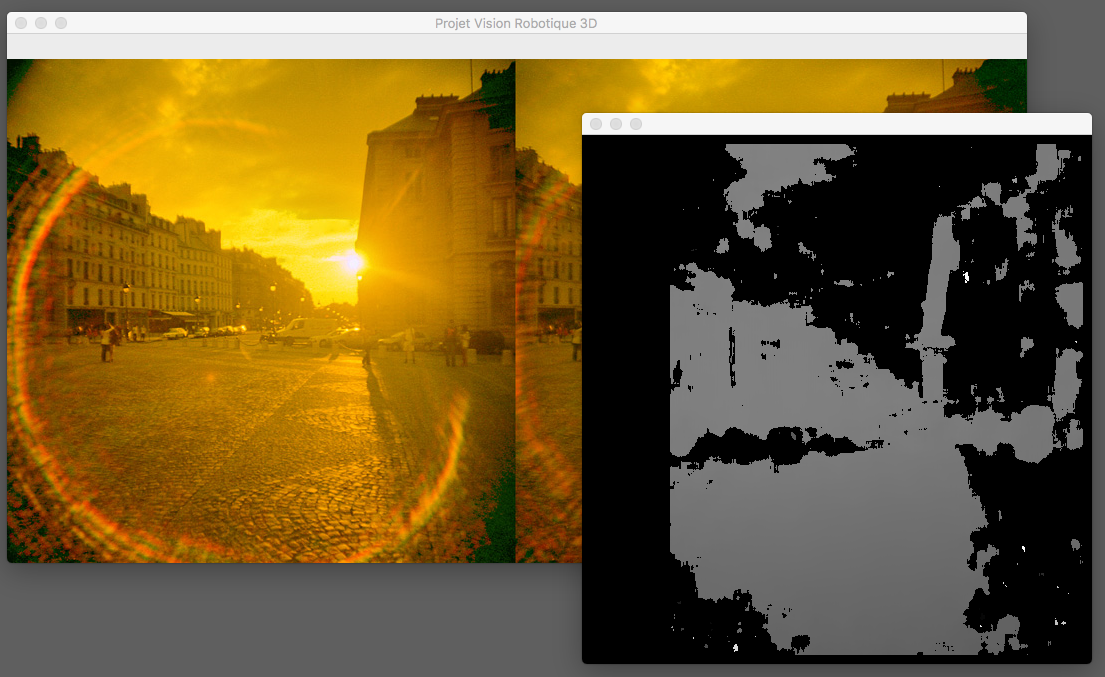
\includegraphics[width=\textwidth,height=\textheight,keepaspectratio]{img/5.png}}

\newpage
\subsection*{Carte de disparité dynamique}

Pour ouvrir l'interface dynamique de calcul de carte de disparité, aller dans le
menu \textbf{Edit} et cliquer sur "SGBM test". Les images chargées sont codées en
dur dans le code. Il n'est donc pas nécessaire d'avoir ouvert une image au préalable. \\
Voici l'interface : \\[0.4cm]

\centerline{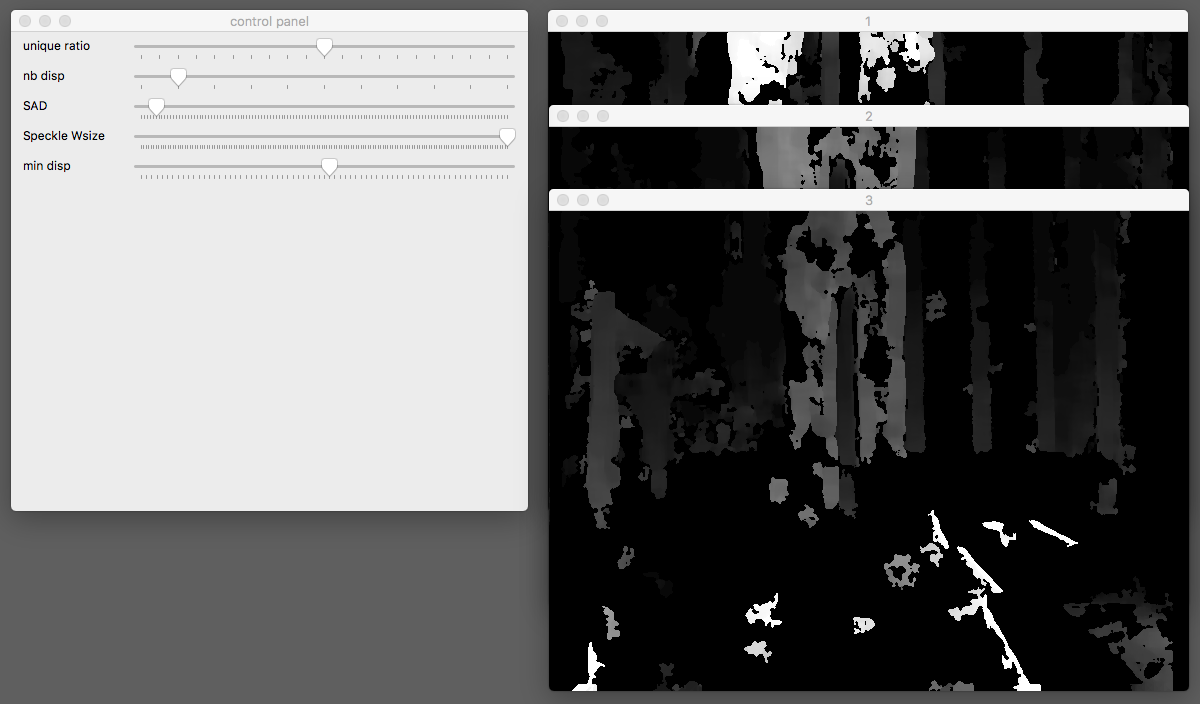
\includegraphics[width=\textwidth,height=\textheight,keepaspectratio]{img/6.png}}

\subsection*{Robot}

N'ayant pas atteint un stade suffisament avancé du développement, aucun test n'a
été effectué sur le robot.

%-------------------------------------------------------------------------------
% Problèmes rencontrés
%-------------------------------------------------------------------------------

\newpage
\section{Problèmes rencontrés}

\subsection*{Installation OpenCV}

Lors des premières séances, nous avons eu des difficultés a installer OpenCV. En effet, utilisant les trois OS majeures(Windows, Mac, Linux), la procédure d'installaion n'était pas la même et nous n'avons pas pu nous aider les uns les autres facilement. Ceci a retardé un peu l'implémentation des fonctions OpenCV, et nous avons même abandonné l'installation sous Windows.

\subsection*{Carte de disparité}

Afin de traiter la carte de disparitée, nous avons dans un premier temps utiliser l'algorithme StereoBM. L'appel à celui-ci sur les images tests fournis par l'enseignant nous retournait un résultat satisfaisant lorsque nous n'utilisions aucun paramètre. Nous avons donc garder cette implémentation naive(pas sur pour cet adjectif) de StereoBM.

Lorsque nous en avons du traiter les images issues du robot, les valeurs par défaut de cet algorithme ne nous donnait pas de résultat concluant. Nous avons donc eu besoin d'implémenter une variation des paramètre de StereoBM dans notre code, afin de mieux controller le résultat. Après avoir essayer pendant plusieurs séances d'améliorer les cartes de profondeur avec cette méthode, nous avons abandonner au profit de l'utilisation de SteroSGBM. Ces deux algorithmes étant similaire dans leur implémentation, nous n'avons pas eu besoin de beaucoup de temps pour adapter notre programme. Nous avons très rapidement obtenu un meilleur résultat avec beaucoup moins d'effort.

\subsection*{Conversion d'images}

Notre conversion d'images a encore des probèmes de source inconnues. En effet, lors de l'appel du split depuis l'interface graphique, les images ne sont pas traités et la fonction split affiche deux fois l'image de gauche. Cependant le split est le seul moment ou nous avont remarqué ce comportement.

%-------------------------------------------------------------------------------
% Conclusion
%-------------------------------------------------------------------------------

\section{Conclusion}

Au travers de ce projet nous avons pu acquérir plusieurs connaissances. Premièrement,
nous avons pu découvrir un nouveau domaine, la reconnaissance visuelle. D'un point
de vue technique, nous avons pu approfondir nos connaissances en C++ et nous avons
également pu apprendre à nous servir d'une libraire open source, OpenCV.
De plus, ce projet présentait un plus par rapport aux autres projets que nous
pouvons réaliser dans le cadre scolaire dans le sens où il permettait d'aller
se confronter aux contraintes physiques.


%-------------------------------------------------------------------------------
% In the end
%-------------------------------------------------------------------------------

\end{document}
